\lecture{Лекция 7}{lec7}
\subtitle{Лекция 7 --- Информационные технологии}

\frame[plain]
{\titlepage}	% Титульный слайд


\begin{frame}
\frametitle{Информационные технологии}

\begin{center}

\Huge
Компьютерные сети
	
\end{center}


\end{frame}

\begin{frame}
\frametitle{Компьютерная сеть}

Компьютерная (вычислительная) сеть --- несколько компьютеров и сетевых устройств, соединенных между собой какой-либо средой передачи данных (Media) для обмена данными.

Узел сети --- компьютер или коммуникационное устройство

Среда передачи данных --- физический канал (проводной или беспроводной), по которому происходит перенос сигналов между отправителем и получателем.

Сегмент сети --- логически или физически обособленная часть сети.
Разбиение сети на сегменты осуществляется с целью оптимизации сетевого трафика и/или повышения безопасности сети в целом. 

\end{frame}

\begin{frame}[t]
\frametitle{Виды компьютерных сетей}

Локальные вычислительные сети (Local Area Network, LAN) 
\begin{itemize}
	\item Линии связи относительно небольшой географической протяженности
	\item Малый процент ошибок передачи данных
	\item Отсутствие механизмов коррекции ошибок
	\item Конечный пункт трафика
\end{itemize}

Глобальные вычислительные сети (Wide Area Network, WAN) 
\begin{itemize}
	\item Сети большой географической протяженности
  \item Технологии (выделенная линия, xDSL, x.25, Frame Relay, MPLS и т.д.)
\end{itemize}

Корпоративные сети --- сети крупных организаций. 

\end{frame}

\begin{frame}[t]
\frametitle{Сетевые устройства}
Сетевой адаптер (Network Interface Card) --- Обеспечивает взаимодействие устройства со средой передачи данных.

Коммутатор (Switch) --- многопортовый повторитель для организации локальных сетей.

Маршрутизатор (Router) --- Обеспечивает передачу данных между сетями


\end{frame}



\begin{frame}[t]
\frametitle{Объединение сегментов сети}
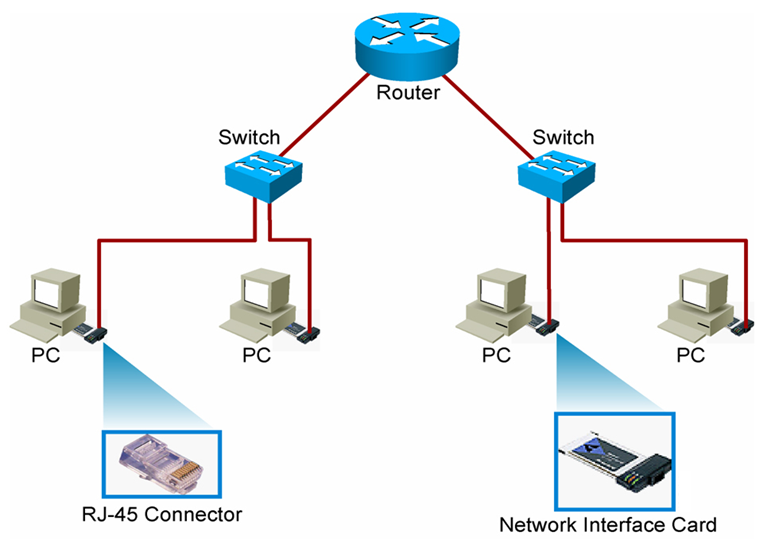
\includegraphics[height=8cm]{images/it_1}

\end{frame}


\begin{frame}[t]
\frametitle{Сетевые топологии }
Физическая топология – способ соединения компьютеров сети
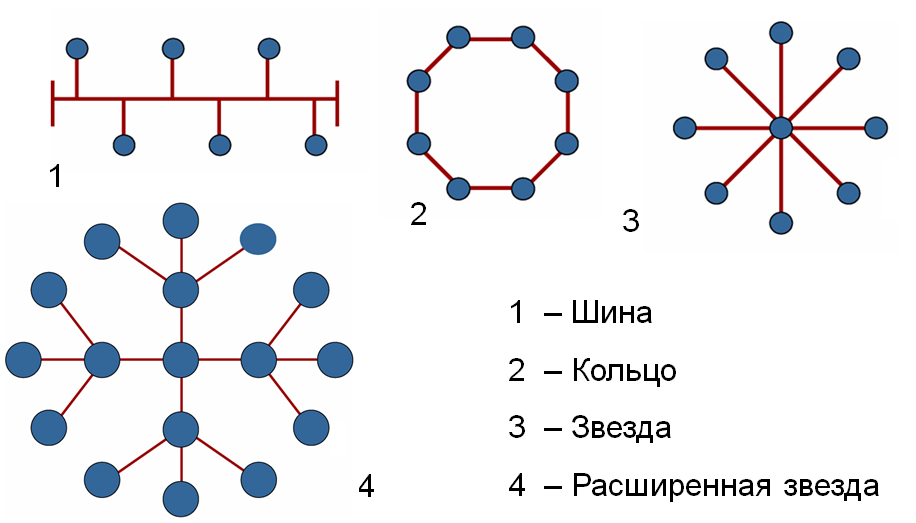
\includegraphics[height=6cm]{images/it_2}


\end{frame}

\begin{frame}[t]
\frametitle{Сетевые топологии }
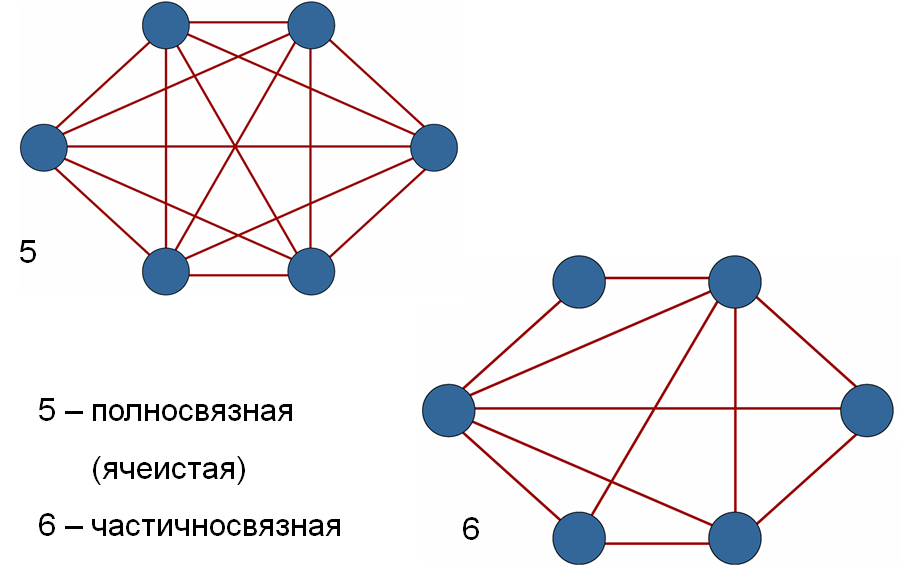
\includegraphics[height=6cm]{images/it_3}


\end{frame}

\begin{frame}[t]
\frametitle{Протоколы}
Сетевой протокол --- набор формальных правил приема и передачи данных (HTTP, FTP и т.п.).

Любой момент сетевого взаимодействия регламентируется каким-либо протоколом.

Стек протоколов (Stack) --- весь комплекс протоколов, обеспечивающих обмен данными (ТСР-IP). 


\end{frame}

\begin{frame}[t]
\frametitle{Адресация в Интернет}
Основным протоколом сети Интернет является сетевой протокол TCP/IP. 

Каждый компьютер, в сети TCP/IP (подключенный к сети Интернет), имеет свой уникальный IP-адрес или IP – номер. 

Адреса в Интернете могут быть представлены как последовательностью цифр, так и именем, построенным по определенным правилам(доменное имя). 

Компьютеры при пересылке информации используют цифровые адреса, а пользователи в работе с Интернетом используют в основном имена.

\end{frame}

\begin{frame}[t]
\frametitle{IP-адрес}
\begin{itemize}
	\item 32-битное двоичное число
\item Четвертая часть адреса – октет или квадрант
\item Визуализация: четыре десятичных числа, 	разделенных точками
\item Идентифицирует сетевой интерфейс на Сетевом 	уровне OSI
\item Две части: адрес (идентификатор) сети и адрес 	(идентификатор) хоста (хост-биты)
\item Хост – сетевой интерфейс
\end{itemize}

192.168.10.2 = $\underbrace{11000000.10101000.0000}_{сеть}\underbrace{1010.00000010}_{узел, хост}$

\end{frame}

\begin{frame}[t]
\frametitle{Зарезервированные IP-адреса}
\begin{itemize}
	\item Адрес сети 192.168.10.0 \\
	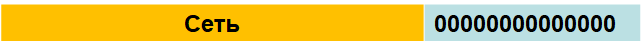
\includegraphics[width=10cm]{images/it_4}
\item Адрес широковещательной рассылки (Broadcast) 192.168.10.255 \\
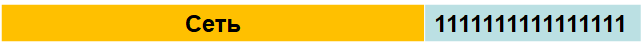
\includegraphics[width=10cm]{images/it_5}

\end{itemize}


\end{frame}

\begin{frame}[t]
\frametitle{Маска подсети}
32-битное двоичное число: $\underbrace{111\ldots111}_{сеть}\underbrace{00\ldots00}_{узел}$

Сокращенная запись – указание количества единичных бит через символ "/" .
Пример:192.168.1.5 255.255.255.0 или 192.168.1.5/24

Формальный механизм выделения частей IP-адреса (побитовая конъюнкция)


\end{frame}

\begin{frame}[t]
\frametitle{Адресное пространство}
Даны IP-адрес и маска сети: 152.215.43.25/21 или 255.255.248.0

По этим значениям определяются:
\begin{itemize}
	\item Количество адресов сети
	\item Количество адресуемых интерфейсов
	\item Адрес сети
	\item Первый и последний адреса сети, допустимые к назначению  на интерфейсы
	\item Адрес широковещательной рассылки
	\item Адрес следующей сети

\end{itemize}



\end{frame}

\begin{frame}[fragile]
\frametitle{Адресное пространство}
Даны IP-адрес и маска сети: 152.215.43.25/21 или 255.255.248.0
\begin{verbatim}
узел  10011000.11010111.00101011.00011001
маска 11111111.11111111.11111000.00000000
сеть  10011000.11010111.00101000.00000000 = 152.215.40.0
\end{verbatim}
Адрес сети : 152.215.40.0 \\
Первый адрес: 152.215.40.1 \\
Широковещательный адрес 
	 00101111.11111111  - 152.215.47.255\\
Последний адрес: 152.215.47.254 \\
Следующая сеть: 152.215.48.0 \\
Количество хостов :$2^{11}-2$ = 2046 \\

\end{frame}

\begin{frame}[fragile]
\frametitle{Универсальный идентификатор ресурсов}
\begin{verbatim}
<схема>:[//<логин>:<пароль>@]<хост>[:<порт>/<URL путь>] 
\end{verbatim}

\textbf{схема}  – способ обращения к ресурсу; в большинстве случаев имеется в виду сетевой протокол;\\
\textbf{логин и пароль} – имя или сетевой псевдоним и пароль пользователя, используемые для доступа к ресурсу;\\
\textbf{хост}  – полностью прописанное доменное имя или IP-адрес хоста (компьютера), на котором располагается ресурс;\\
\textbf{порт}  – номер, связанный с приложением;\\
\textbf{URL путь}  – уточняющая информация о месте нахождения ресурса (зависит от протокола);

\begin{verbatim}
http://cs.msu.ru/entrance/questions.html
\end{verbatim}


\end{frame}

\begin{frame}[fragile]
\frametitle{Задачи}
Задача 1: По данным IP-адресу 152.215.43.25 и маске сети 255.255.248.0 найти порядковый номер компьютера в сети.
\pause Ответ 793

Задача 2:  Два узла, находящиеся в одной сети, имеют IP-адреса 118.222.130.140 и 118.222.201.140. Укажите наибольшее возможное значение третьего слева байта маски сети. Ответ запишите в виде десятичного числа.

\pause Ответ 128
\end{frame}


\begin{frame}
\frametitle{Информационные технологии}

\begin{center}

\Huge
Электронные таблицы
	
\end{center}

\end{frame}


\begin{frame}[fragile]
\frametitle{Электронные таблицы }
Электронные таблицы (ЭТ) --- компьютерная программа, позволяющая автоматизировать вычисления с большими объёмами данных, представленных в виде двумерных таблиц.

\textbf{Рабочая книга} – документ, создаваемый электронными таблицами.\\
\textbf{Рабочая книга} состоит из рабочих листов – отдельных электронных таблиц, между которыми возможен обмен данными. \\
\textbf{Рабочий лист} состоит из \textbf{ячеек}. 

Различают: адрес ячейки и содержимое ячейки.

\end{frame}

\begin{frame}[fragile]
\frametitle{Формулы}
\textbf{Формула} - выражение, с помощью которого вычисляется новое значение на основании имеющихся.\\
Формула начинается с символа <<=>>;\\
Формула может содержать: 
\begin{itemize}
\item константы;
\item функции;
\item ссылки.

\end{itemize}


\end{frame}

\begin{frame}[fragile]
\frametitle{Виды ссылок}
\textbf{Относительная ссылка}: – смещение относительно рабочей клетки до клетки, откуда нужно взять данные. \\
Относительные ссылки в формуле выглядят как адреса ячеек.

Например: В ячейке B5 содержится формула <<=D2>>.

Это значит, что В5 ссылается на ячейку расположенную на 2 столбца правее и на 3 строки выше.

При копировании формулы относительные ссылки автоматически пересчитываются.




\end{frame}

\begin{frame}[fragile]
\frametitle{Виды ссылок}

\textbf{Абсолютная ссылка} – ссылка на фиксированную ячейку рабочего листа. В формуле визуально отличает-ся наличием двух символов \$ перед заголовком строки и номером столбца. Например: \$A\$4

\textbf{Смешанная ссылка } --- ссылка, в которой зафиксирована одна из частей. Например: А\$1 или \$А1
\end{frame}


\begin{frame}[fragile]
\frametitle{Задачи}

Задача 1.	В ячейки диапазона C3:F6 электронной таблицы записаны числа, как показано на рисунке.
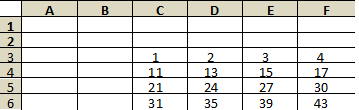
\includegraphics[width=10cm]{images/it_6}

В ячейке A1 записали формулу =E$5-$D4. После этого ячейку A1 скопировали в ячейку B2. Какое число будет показано в ячейке B2? Примечание: знак \$ используется для обозначения абсолютной адресации.

\pause 
Ответ 1

\end{frame}

\begin{frame}[fragile]
\frametitle{Задачи}

Задача 2.	Задача: Дан фрагмент электронной таблицы. Какое чис-ло должно быть записано в ячейке B1, чтобы построенная после вычислений диаграмма по значениям диапазона ячеек A2:C2 соответствовала рисунку. Известно, что все значения диапазона, по которому построена диаграмма, имеют один и тот же знак.
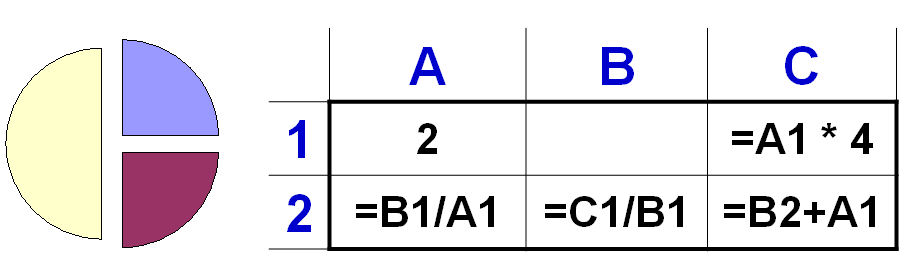
\includegraphics[width=10cm]{images/it_7}

\pause 
Ответ 4

\end{frame}


\begin{frame}
\frametitle{Информационные технологии}

\begin{center}

\Huge
Хранение  и  поиск информации в базах данных.
	
\end{center}

\end{frame}


\begin{frame}[fragile]
\frametitle{Задачи}

\textbf{База данных} (БД) --- разновидность информационной системы, предоставляющей функции централизован-ного  хранения и накопления логически связанных  данных в соответствии с реализованной моделью в вычислительной системе.

\textbf{Модель данных} – формальный способ представления данных в СУБД.

\textbf{Система управления базами данных} (СУБД) – специализированный пакет программ, обеспечивающий возможность организации и ведения базы данных.


\end{frame}

\begin{frame}[fragile]
\frametitle{Реляционная модель}

Данные организованы в виде двумерных таблиц.
Модель предложена Эдгаром Коддом в 1970 году. 

\textbf{Достоинства}: простота, понятность и удобство реализации на ЭВМ.

\textbf{Недостатки}: не допускает естественного представления данных со сложной структурой, что ведёт к временным потерям на их обработку.

\end{frame}

\begin{frame}[fragile]
\frametitle{Основные понятия для реляционной модели}

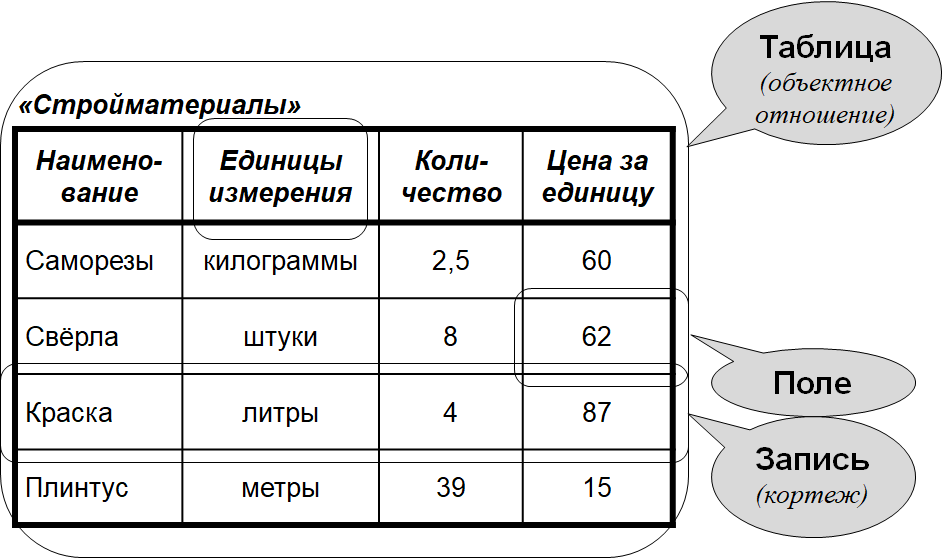
\includegraphics[width=10cm]{images/it_8}

\end{frame}

\begin{frame}[fragile]
\frametitle{Задачи}
\small
Задача 1. На основании приведённых данных определите, сколько прямых потомков (т.е. детей и внуков) Павленко А.К. упомянуты в таблице 1.\\
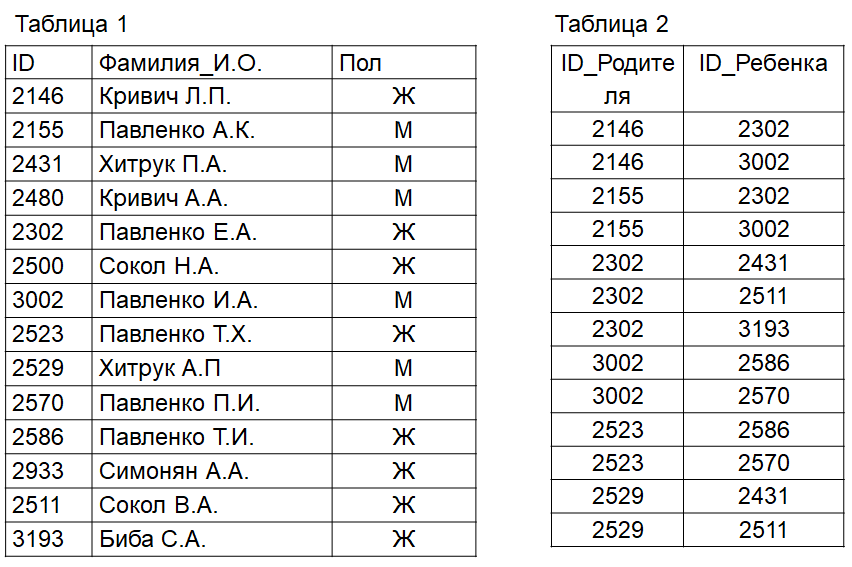
\includegraphics[height=6cm]{images/it_9}\pause  Ответ 7
\end{frame}

\begin{frame}
\frametitle{Информационные технологии}

\begin{center}

\Huge
Файловая система
	
\end{center}

\end{frame}

\begin{frame}
\frametitle{Интерфейс файловой системы}

Файловая система является важной и хорошо видимой частью операционной системы.

Это больше, чем просто способ хранения данных и программ.

Он также обеспечивает организацию файлов через структуру каталогов и поддерживает метаданные, связанные с файлами.

Основное взаимодействие пользователя с ОС это работа с файловой системой.

\end{frame}

\begin{frame}
\frametitle{Что такое файл?}

Но что такое файл? Ответ ОС таков: \alert{Все есть файл!}

Что касается компьютера, любые данные это набор нулей и единиц.

Файл просто логическая единица, чтобы организовать данные.

Таким образом, область диска обозначается как принадлежащая файлу.
\end{frame}

\begin{frame}
\frametitle{Что такое файл?}

Файлы могут содержать программы (например, \texttt{word.exe}) и/или данные (например, \texttt{report.doc}).

Содержимое файла определяется его создателем.

Создатель может быть пользователем, если он или она использует блокнот или что-то, или это может быть программа, например компилятор, создающий выходной двоичный файл.

\end{frame}

\begin{frame}[fragile]
\frametitle{Виды файлов}
\begin{itemize}
\item{Каталоги}
\item{Файлы
  \begin{itemize}
    \item{Символьные специальные файлы (моделирование последовательных устройств ввода-вывода)}
    \item{Блочные специальные файлы (моделирование дисков)}
		 \item{Обычные файлы
		  \begin{itemize}
			\item{Бинарные (исполнимые)}
			\item{Текстовые
			\begin{verbatim}
			   Текстовые
			   Типизированные (видео, архив)
			   Шелл-коды
			\end{verbatim}
			}
			\end{itemize}
		}
\end{itemize}

}
\end{itemize}
\end{frame}

\begin{frame}
\frametitle{Атрибуты файла}

Файлы, как правило, имеют атрибуты, которые обычно включают в себя следующее:

\begin{enumerate}
	\item \textbf{Имя файла}
	\item \textbf{Идентификатор}
	\item \textbf{Тип}
	\item \textbf{Расположение}
	\item \textbf{Размер}
	\item \textbf{Защита}
	\item \textbf{Время, Дата, UserID}
\end{enumerate}


\end{frame}

\begin{frame}
\frametitle{Структура каталогов}

Файлы хранятся в структуре каталогов.

Структура каталогов нам хорошо знакома как папки в системе.

Каталоги действительно похожи на файлы: они являются информацией о том, какие файлы находятся в каких местах, и они тоже будут храниться на диске.

\end{frame}

\begin{frame}[fragile]
\frametitle{Полное имя файла}
OC идентифицирует файл по полному имени.
Полное имя файла состоит из трёх частей:
\begin{itemize}
	\item имя устройства;
	\item путь к файлу;
	\item имя файла.
\end{itemize}

\textbf{Путь к файлу} – последовательность имен каталогов, разделенных символом <<$\backslash$>> указывающая расположение файла в файловой системе.
Пример полного имени файла:
\begin{verbatim}
C:\WINDOWS\SYSTEM32\version.dll
\end{verbatim}

\end{frame}

\begin{frame}[fragile]
\frametitle{Путь к файлу}
\textbf{Абсолютный путь} --- путь, начинающийся от корневого каталога. \\
\textbf{Текущий каталог} --- каталог, с которого начинается поиск файлов, если явно не указано другое.
\textbf{Относительный путь} --- путь, начинающийся от текущего каталога.

Стандартное имя текущего каталога – символ <<.>>
Подкаталог – каталог, находящийся внутри другого каталога. 

\textbf{Родительский} (материнский) каталог – каталог, в котором содержится рассматриваемый каталог.
Стандартное имя родительского каталога – два символа  <<..>>

\end{frame}

\begin{frame}[fragile]
\frametitle{Шаблоны (маски) имён файлов}
Шаблон (маска) имен файлов --- метод описания имен с применением символов маскирования.

Символы-маскирования:\\
«*» – заменяет произвольную последовательность символов;\\
«?» – заменяет ровно один любой символ.

\end{frame}

\begin{frame}[fragile]
\frametitle{Задачи}
Задача. В каталоге находится 6 файлов:
omerta.doc; chimera.dat; chimera.doc; izmeren.doc; mesmer.docx; k-mer-list.doc

Определите, по какой из масок из каталога будет
отобрана такая группа файлов:\\
omerta.doc\\
chimera.doc\\
izmeren.doc\\
k-mer-list.doc

1) *mer?*.d*	2) *?mer*?.do*	3) ?mer*.doc	4) *mer?.doc*\\
\pause Ответ 2

\end{frame}



